\documentclass[tikz,border=8pt]{standalone}
\usepackage{pgfplots}
\usepackage{pgfplotstable}
\usetikzlibrary{pgfplots.groupplots,positioning}
\pgfplotsset{compat=1.18}

\definecolor{attrblue}{RGB}{136,186,228}
\definecolor{attrred}{RGB}{230,152,145}
\definecolor{attrgray}{RGB}{200,205,214}
\definecolor{notegray}{RGB}{245,247,250}
\definecolor{noteline}{RGB}{210,214,220}

\begin{document}
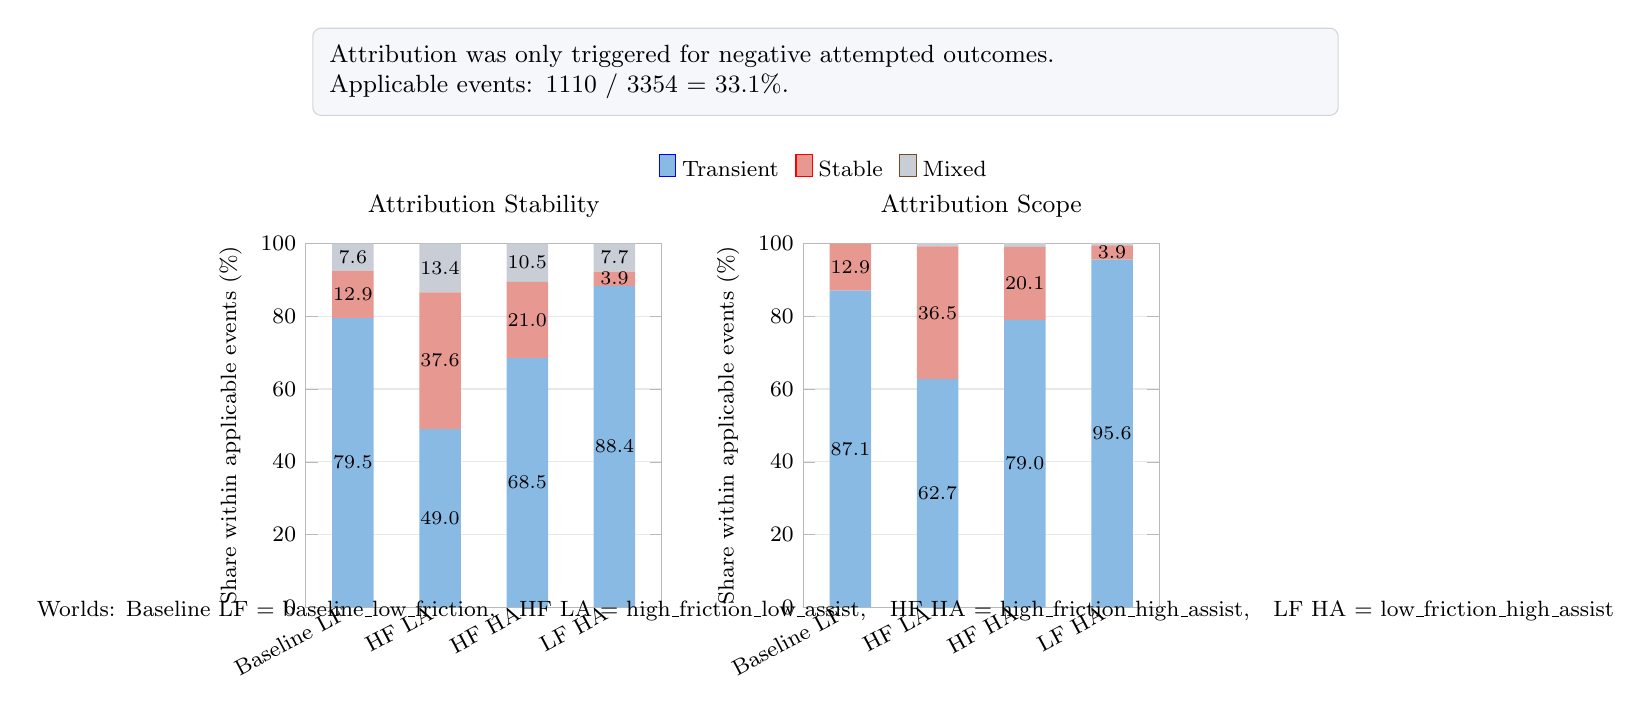
\begin{tikzpicture}
  \node[
    draw=noteline,
    fill=notegray,
    rounded corners=3pt,
    align=left,
    inner sep=6pt,
    text width=12.6cm,
    font=\small
  ] (note) at (6.6,6.8) {Attribution was only triggered for negative attempted outcomes.\\
  Applicable events: 1110 / 3354 = 33.1\%.};

  \begin{groupplot}[
    group style={group size=2 by 1, horizontal sep=1.8cm},
    width=6.1cm,
    height=6.2cm,
    ymin=0,
    ymax=100,
    ybar stacked,
    symbolic x coords={Baseline LF,HF LA,HF HA,LF HA},
    xtick=data,
    enlarge x limits=0.18,
    ylabel={Share within applicable events (\%)},
    tick label style={font=\footnotesize},
    label style={font=\footnotesize},
    title style={font=\small},
    x tick label style={rotate=28,anchor=east,font=\footnotesize},
    ymajorgrids=true,
    grid style={draw=gray!18},
    axis line style={draw=gray!55},
    tick style={draw=gray!55},
    legend style={
      draw=none,
      fill=none,
      font=\footnotesize,
      legend columns=3,
      /tikz/every even column/.append style={column sep=4pt}
    },
    nodes near coords,
    every node near coord/.append style={font=\scriptsize, text=black},
    point meta=explicit symbolic
  ]

    \nextgroupplot[
      title={Attribution Stability},
      legend to name=attrlegend
    ]
      \addplot+[draw=none, fill=attrblue, bar width=15pt]
        coordinates {
          (Baseline LF,79.5) [79.5]
          (HF LA,49.0) [49.0]
          (HF HA,68.5) [68.5]
          (LF HA,88.4) [88.4]
        };
      \addplot+[draw=none, fill=attrred, bar width=15pt]
        coordinates {
          (Baseline LF,12.9) [12.9]
          (HF LA,37.6) [37.6]
          (HF HA,21.0) [21.0]
          (LF HA,3.9) [3.9]
        };
      \addplot+[draw=none, fill=attrgray, bar width=15pt]
        coordinates {
          (Baseline LF,7.6) [7.6]
          (HF LA,13.4) [13.4]
          (HF HA,10.5) [10.5]
          (LF HA,7.7) [7.7]
        };
      \legend{Transient,Stable,Mixed}

    \nextgroupplot[
      title={Attribution Scope}
    ]
      \addplot+[draw=none, fill=attrblue, bar width=15pt]
        coordinates {
          (Baseline LF,87.1) [87.1]
          (HF LA,62.7) [62.7]
          (HF HA,79.0) [79.0]
          (LF HA,95.6) [95.6]
        };
      \addplot+[draw=none, fill=attrred, bar width=15pt]
        coordinates {
          (Baseline LF,12.9) [12.9]
          (HF LA,36.5) [36.5]
          (HF HA,20.1) [20.1]
          (LF HA,3.9) [3.9]
        };
      \addplot+[draw=none, fill=attrgray, bar width=15pt]
        coordinates {
          (Baseline LF,0.0) [0.0]
          (HF LA,0.9) [0.9]
          (HF HA,1.0) [1.0]
          (LF HA,0.6) [0.6]
        };
  \end{groupplot}

  \node[anchor=north, font=\footnotesize] at (6.6,0.2) {
    Worlds: Baseline LF = baseline\_low\_friction,\quad HF LA = high\_friction\_low\_assist,\quad HF HA = high\_friction\_high\_assist,\quad LF HA = low\_friction\_high\_assist
  };

  \node[anchor=north] at (6.6,5.95) {\pgfplotslegendfromname{attrlegend}};
\end{tikzpicture}
\end{document}
